\ExamPart{Trắc nghiệm nhiều phương án lựa chọn}{3.0}{Thí sinh trả lời từ câu 1 đến câu 12. Mỗi câu thí sinh chỉ chọn một phương án.}

\NQuestion Cho đồ thị hàm số $y=f(x)$ như hình vẽ dưới đây.
\begin{center}
    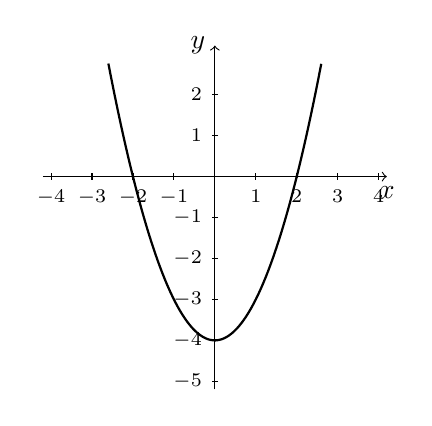
\begin{tikzpicture}[scale=0.52]
    \draw[->] (-4.2,0) -- (4.2,0) node[below] {$x$};
    \draw[->] (0,-5.2) -- (0,3.2) node[left] {$y$};
    \foreach \x in {-4,-3,-2,-1,1,2,3,4}
      \draw (\x,0.08)--(\x,-0.08) node[below] {\scriptsize $\x$};
    \foreach \y in {-5,-4,-3,-2,-1,1,2}
      \draw (0.08,\y)--(-0.08,\y) node[left] {\scriptsize $\y$};
    \draw[smooth, samples=200, domain=-2.6:2.6, thick] plot (\x, {\x*\x-4});
    \fill (-2,0) circle (1.2pt);
    \fill (2,0) circle (1.2pt);
    \fill (0,-4) circle (1.2pt);
\end{tikzpicture}

\end{center}
Tập nghiệm của bất phương trình $f(x)\le 0$ là
\ChoicesOneLine
{$[-2;2]$.}
{$(-\infty;-2]\cup[2;+\infty)$.}
{$(-2;2)$.}
{$(-\infty;-2)\cup(2;+\infty)$.}
{1}
\SolutionBlock{Từ đồ thị, parabol mở lên và cắt trục hoành tại $x=-2$, $x=2$. Vì vậy $f(x)\le0$ khi $x\in[-2;2]$.}

\NQuestion Cho đồ thị hàm số $y=f(x)$ như hình vẽ dưới đây.
\begin{center}
    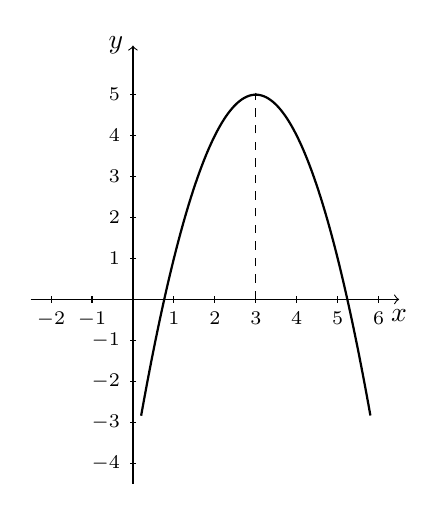
\begin{tikzpicture}[scale=0.52]
    \draw[->] (-2.5,0) -- (6.5,0) node[below] {$x$};
    \draw[->] (0,-4.5) -- (0,6.2) node[left] {$y$};
    \foreach \x in {-2,-1,1,2,3,4,5,6}
      \draw (\x,0.08)--(\x,-0.08) node[below] {\scriptsize $\x$};
    \foreach \y in {-4,-3,-2,-1,1,2,3,4,5}
      \draw (0.08,\y)--(-0.08,\y) node[left] {\scriptsize $\y$};
    \draw[smooth, samples=200, domain=0.2:5.8, thick] plot (\x, {-(\x-3)*(\x-3)+5});
    \draw[dashed] (3,0) -- (3,5);
    \fill (3,5) circle (1.2pt);
\end{tikzpicture}

\end{center}
Giá trị lớn nhất của hàm số trên đoạn $[1;5]$ là
\ChoicesOneLine{$3$.}{$4$.}{$5$.}{$6$.}{3}
\SolutionBlock{Từ đồ thị, parabol mở xuống, đỉnh là điểm cao nhất và có tọa độ $(3;5)$. Do đó giá trị lớn nhất trên đoạn $[1;5]$ là $5$.}

\NQuestion Tập nghiệm của bất phương trình $x^2-7x+12<0$ là
\ChoicesOneLine
{$(-\infty;3)\cup(4;+\infty)$.}
{$(3;4)$.}
{$[3;4]$.}
{$(-\infty;3]\cup[4;+\infty)$.}
{2}
\SolutionBlock{Ta có $x^2-7x+12=(x-3)(x-4)$. Vì hệ số $a>0$ nên tam thức âm giữa hai nghiệm. Suy ra tập nghiệm là $(3;4)$.}

\NQuestion Phương trình $\sqrt{2x+3}=x+1$ có nghiệm là
\ChoicesOneLine{$x=1$.}{$x=\dfrac{1+\sqrt{13}}{2}$.}{$x=1$ hoặc $x=-1$.}{vô nghiệm.}{1}
\SolutionBlock{Điều kiện $x\ge -1$. Bình phương hai vế:
\[
2x+3=(x+1)^2 \Leftrightarrow x^2-1=0 \Leftrightarrow x=\pm1.
\]
Thử lại, $x=1$ thỏa mãn còn $x=-1$ không thỏa. Vậy phương trình có nghiệm $x=1$.}

\NQuestion Một tổ có $6$ học sinh nam và $5$ học sinh nữ. Số cách chọn $1$ nam và $1$ nữ để trực nhật là
\ChoicesOneLine{$11$.}{$30$.}{$36$.}{$60$.}{2}
\SolutionBlock{Theo quy tắc nhân, số cách chọn là $6\cdot5=30$.}

\NQuestion Trong mặt phẳng tọa độ $Oxy$, cho $A(-1;2)$, $B(4;-3)$. Tọa độ của vectơ $\overrightarrow{AB}$ là
\ChoicesOneLine{$(3;-1)$.}{$(5;-5)$.}{$(-5;5)$.}{$(5;1)$.}{2}
\SolutionBlock{Ta có $\overrightarrow{AB}=(4-(-1);-3-2)=(5;-5)$.}

\NQuestion Đường tròn có tâm $I(2;-1)$ và bán kính $R=3$ có phương trình là
\ChoicesOneLine
{$(x-2)^2+(y+1)^2=9$.}
{$(x+2)^2+(y-1)^2=9$.}
{$(x-2)^2+(y-1)^2=3$.}
{$(x+2)^2+(y+1)^2=9$.}
{1}
\SolutionBlock{Phương trình đường tròn tâm $I(a;b)$ bán kính $R$ là $(x-a)^2+(y-b)^2=R^2$. Thay $a=2,b=-1,R=3$ được $(x-2)^2+(y+1)^2=9$.}

\NQuestion Đường thẳng đi qua điểm $M(1;2)$ và có vectơ pháp tuyến $\vec n=(2;-3)$ là
\ChoicesOneLine
{$2x-3y+4=0$.}
{$2x+3y-8=0$.}
{$3x+2y-7=0$.}
{$2x-3y+1=0$.}
{1}
\SolutionBlock{Phương trình đường thẳng là $2(x-1)-3(y-2)=0\Leftrightarrow 2x-3y+4=0$.}

\NQuestion Khoảng cách từ điểm $P(1;-2)$ đến đường thẳng $d:2x-y+5=0$ bằng
\ChoicesOneLine{$1$.}{$\dfrac{9}{\sqrt5}$.}{$\dfrac{5}{\sqrt5}$.}{$\dfrac{1}{\sqrt5}$.}{2}
\SolutionBlock{Ta có
\[
d(P,d)=\dfrac{|2\cdot1-(-2)+5|}{\sqrt{2^2+(-1)^2}}=\dfrac{9}{\sqrt5}.
\]}

\NQuestion Giá trị của biểu thức $A_7^2$ bằng
\ChoicesOneLine{$14$.}{$21$.}{$42$.}{$49$.}{3}
\SolutionBlock{Ta có $A_7^2=7\cdot6=42$.}

\NQuestion Xét bất phương trình $x^2-2mx+m^2-4<0$. Khẳng định nào sau đây đúng về tập nghiệm của bất phương trình?
\ChoicesOneLine
{$m=0$.}
{$m=1$.}
{$m\in\mathbb R$.}
{$m$ là số nguyên dương.}
{3}
\SolutionBlock{Ta có
\[
x^2-2mx+m^2-4=(x-m)^2-4.
\]
Bất phương trình tương đương
\[
(x-m)^2<4 \Leftrightarrow -2<x-m<2 \Leftrightarrow m-2<x<m+2.
\]
Kết quả đúng với mọi $m\in\mathbb R$. Đây là câu vận dụng cao.}

\NQuestion Trong mặt phẳng tọa độ $Oxy$, cho ba điểm $A(1;2)$, $B(5;2)$, $C(3;6)$. Bán kính đường tròn ngoại tiếp tam giác $ABC$ bằng
\ChoicesOneLine{$\dfrac{5}{2}$.}{$2\sqrt5$.}{$\sqrt5$.}{$4$.}{1}
\SolutionBlock{Ta có $AB=4$, trung điểm của $AB$ là $I(3;2)$. Vì $C(3;6)$ có cùng hoành độ với $I$ nên $CI\perp AB$ và $CA=CB=\sqrt{(3-1)^2+(6-2)^2}=2\sqrt5$. Tam giác cân tại $C$ với đáy $AB=4$.
Mặt khác tam giác $ABC$ vuông tại $C$? Không, vì $CA^2+CB^2=40\ne16$. Ta tìm tâm ngoại tiếp là giao của trung trực $AB$ và trung trực $AC$.
Trung trực của $AB$ là $x=3$. Trung điểm của $AC$ là $(2;4)$, hệ số góc $AC=2$ nên trung trực $AC$ có hệ số góc $-\dfrac12$: 
\[
y-4=-\dfrac12(x-2).
\]
Thế $x=3$ được $y=\dfrac72$. Tâm là $O(3;\tfrac72)$.
Do đó
\[
R=OA=\sqrt{(3-1)^2+\left(\dfrac72-2\right)^2}=\sqrt{4+\dfrac94}=\dfrac52.
\]
}
